
%%%%%%%%%%%%%%%%%%%%%%%%%%%%%%%%%%%%%%%%%%%%%%%%%%%%%%%%%%%%%%%%%%%%%%%%
% Approach
%%%%%%%%%%%%%%%%%%%%%%%%%%%%%%%%%%%%%%%%%%%%%%%%%%%%%%%%%%%%%%%%%%%%%%%%
\section{Proposed Approach}
\label{sec:method}

%\note{This intro here must be much more concrete, it is too general and high level. Also, it is very long.}

 \begin{figure}[t]
 \centering
 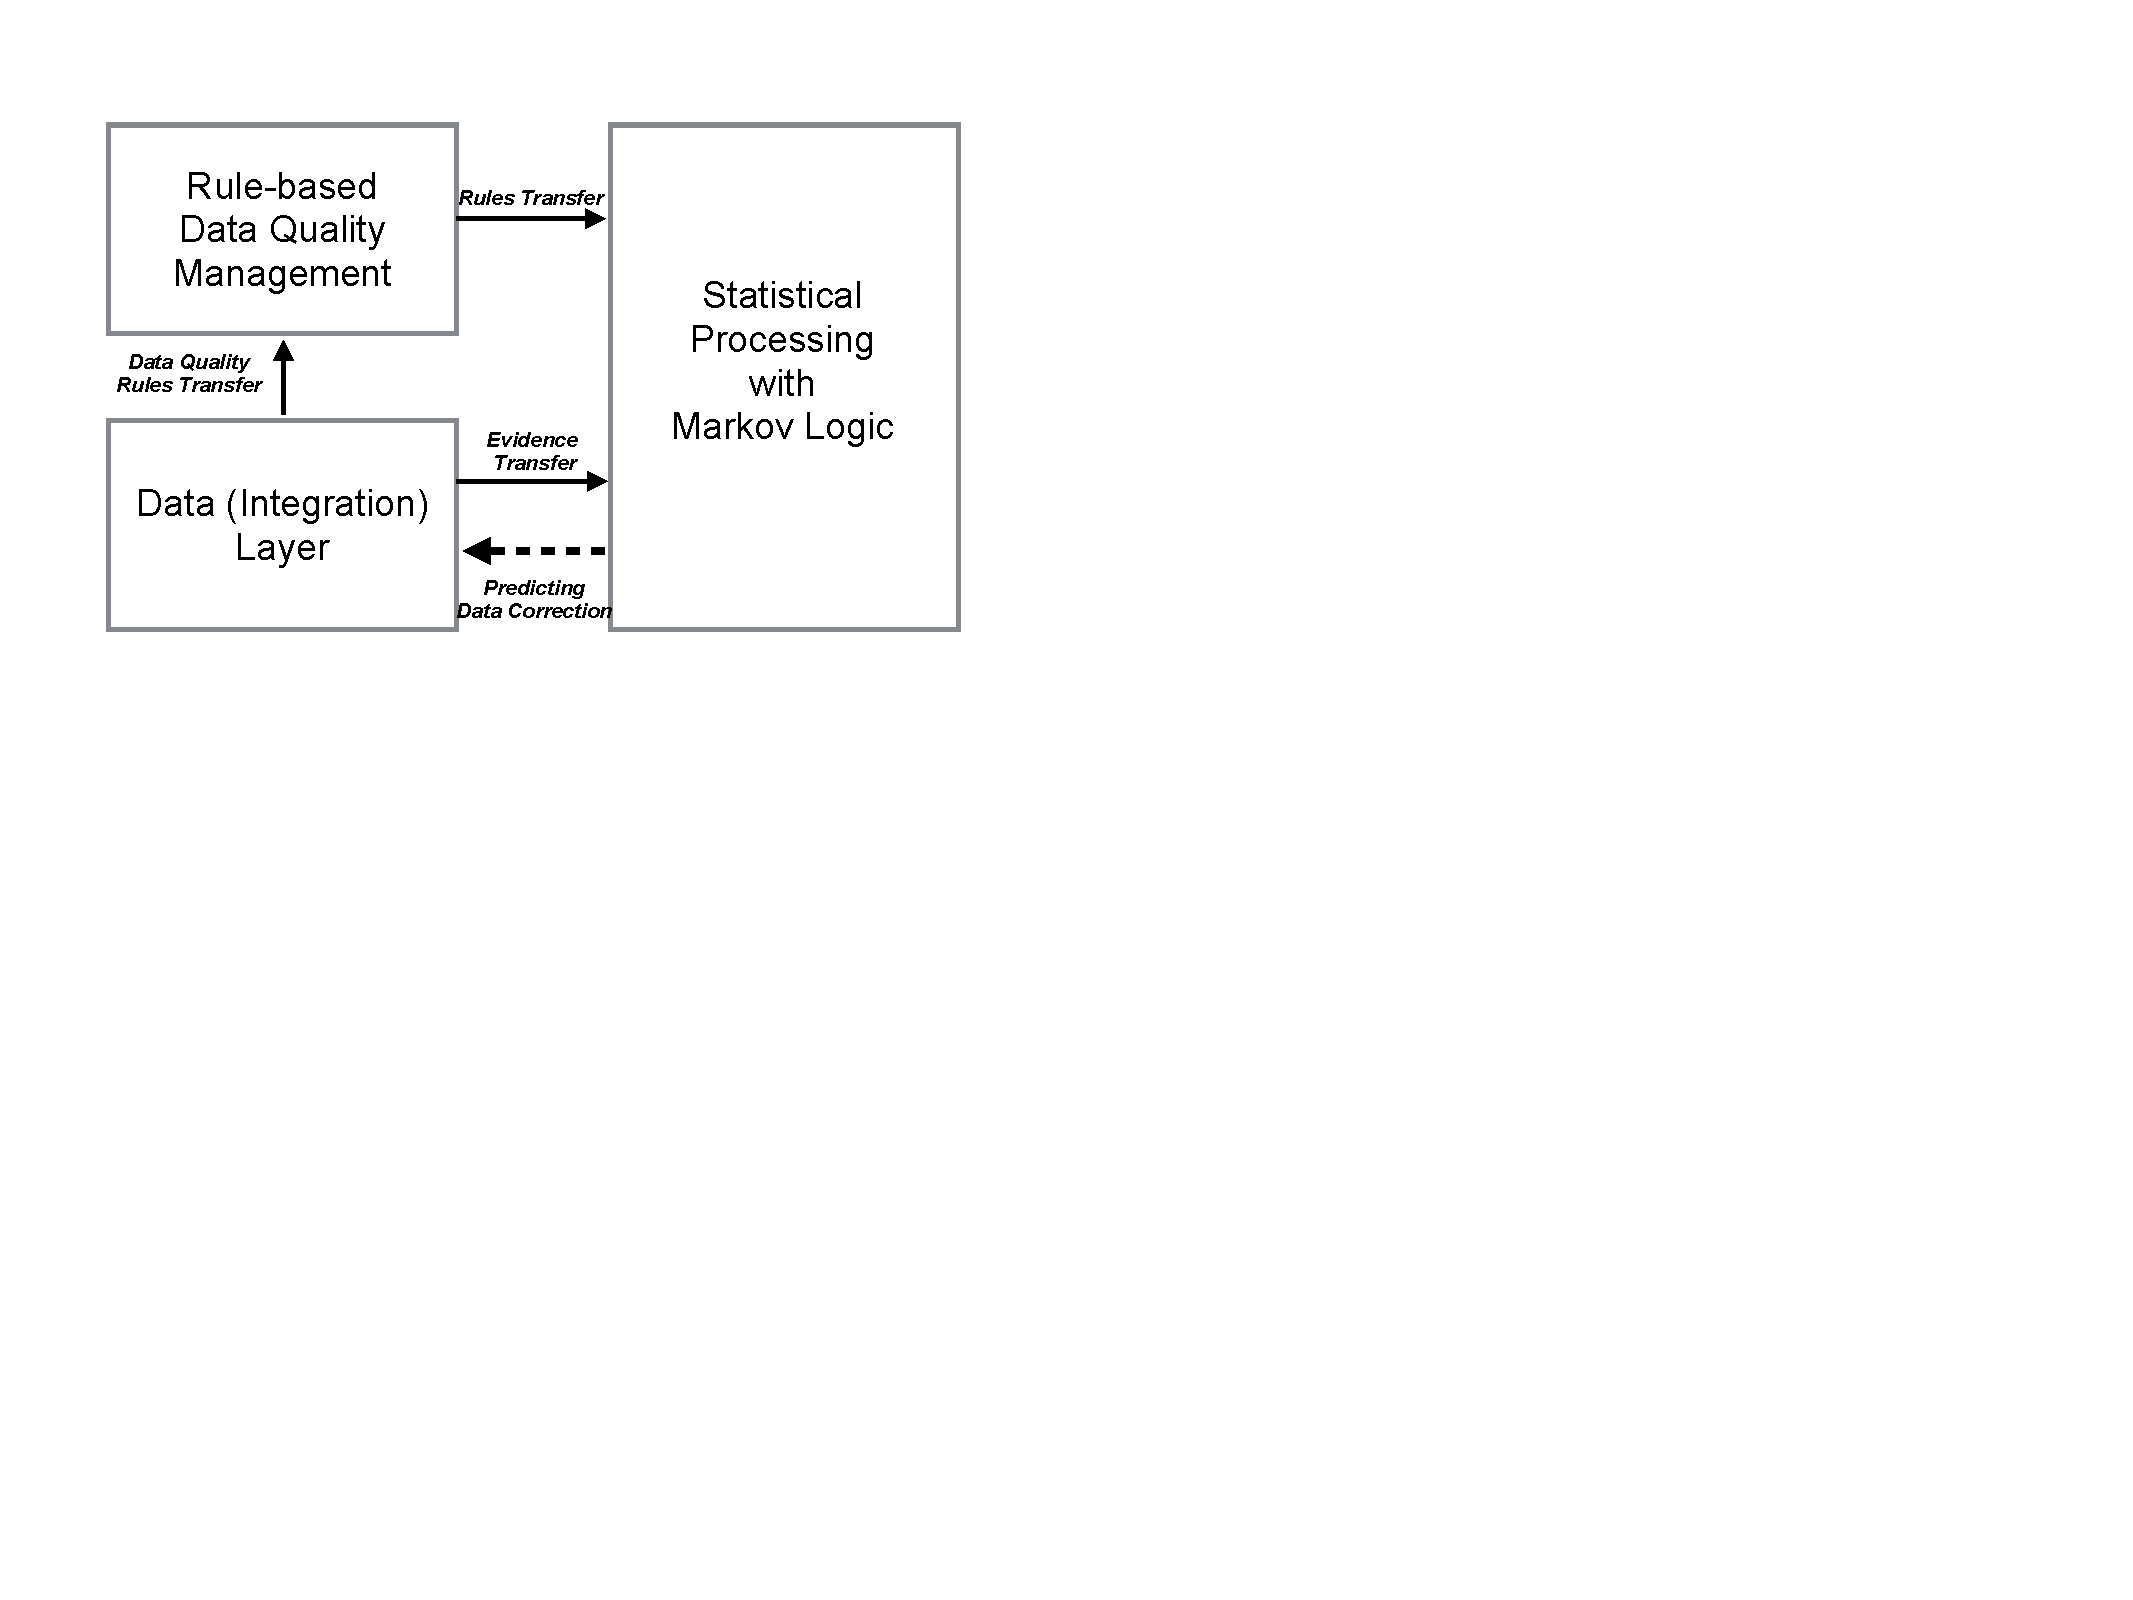
\includegraphics[width=200px, height=140px]{img/system.pdf}
 \caption{%\anno{Rmove this picture?} Why? I find this pic useful and supports understanding.
 \anno{Please redo this picture to make it look better (e.g., make sure the margins of text to borders are always the same.)} Our proposed method for data cleaning based on Markov logic consists of three main components: 
 (I) A \textbf{Rule-based Data Quality Management} component that is based on the data quality rules to address different data quality issues;
 (II) A \textbf{relation prediction} component based on probabilistic inference performed by the Markov logic framework and (III) 
 a \textbf{Data Layer} that includes a number of data sources including relational and semi-structured data.}
 \label{fig:system}
\end{figure}     

We propose to model data cleaning rules in the \textit{Markov logic}~\cite{domingos2009markov} formalism and use probabilistic inference for data cleaning. Markov logic is a knowledge representation system that combines first-order logic as a declarative language and probabilistic graphical models (undirected Markov Networks) on top of which we perform probabilistic inference. We introduce technical aspects of Markov Logic and joint inference for data cleaning in Section~\ref{subsec:jointinference}

The main advantage of Markov logic is the ability to reason simultaneously about complex and interacting relationships. By modeling different data cleaning rules as Markov logic program we leverage the joint inference on underlying probabilistic graphical model. In this way, we implement \textit{holistic} data cleaning, which is one of main requirements for the data cleaning systems \cite{fan2013data, Fan:2014:IRM:2628135.2567657, Dallachiesa:2013:NCD:2463676.2465327}. If no perfect resolution of a ruleset is possible, we want to find data cleaning steps that fulfill as many rules as possible while violating only a few~\cite{genesereth1987logical, domingos2009markov}. Therefore, in order to infer the types of errors and their sources, we consider integrity constraints to be probabilistic. We build on an existing approach to specify \textit{"soft"} functional dependencies between columns~\cite{Ilyas:2004:CAD:1007568.1007641}. 

Another advantage of Markov Logic is that it allows us to tackle overfitting, a common problem when applying machine learning for repairing errorneous data \anno{You still need to explain overfitting!, EDBT reviewers might not be ML experts}. Overfitting occurs when one applies data quality rules that hold only for a fraction of data, but do not hold globally. Markov logic programs with \textit{"soft"} rules prohibit overfitting by adding weights to the constaint-based rules and incorporating partial knowledge \cite{singla2006entity, poon2008joint, lowd2007recursive}. \note{one more sentence, how does adding weights prohibit overfitting? do we show this experimentally somehow? if not, we might want to remove this paragraph}. Furthermore, Markov Logic enables us to extend traditional data quality rules with semantic constraints~\cite{spies2013knowledge}. \note{explain this in more detail, I don't understand what you mean}



In the following, we illustrate how to transfer data cleaning rules into Markov Logic and leverage probabilistic inference to determine data repair operations for a given dataset. \anno{See also Figure \ref{fig:system} for high-level overview of our method-workflow.} \note{YOU NEED TO EXPLAIN FIGURES, NOT JUST REFERENCE THEM *PEITSCH*}


\begin{figure*}[t]
 \centering
 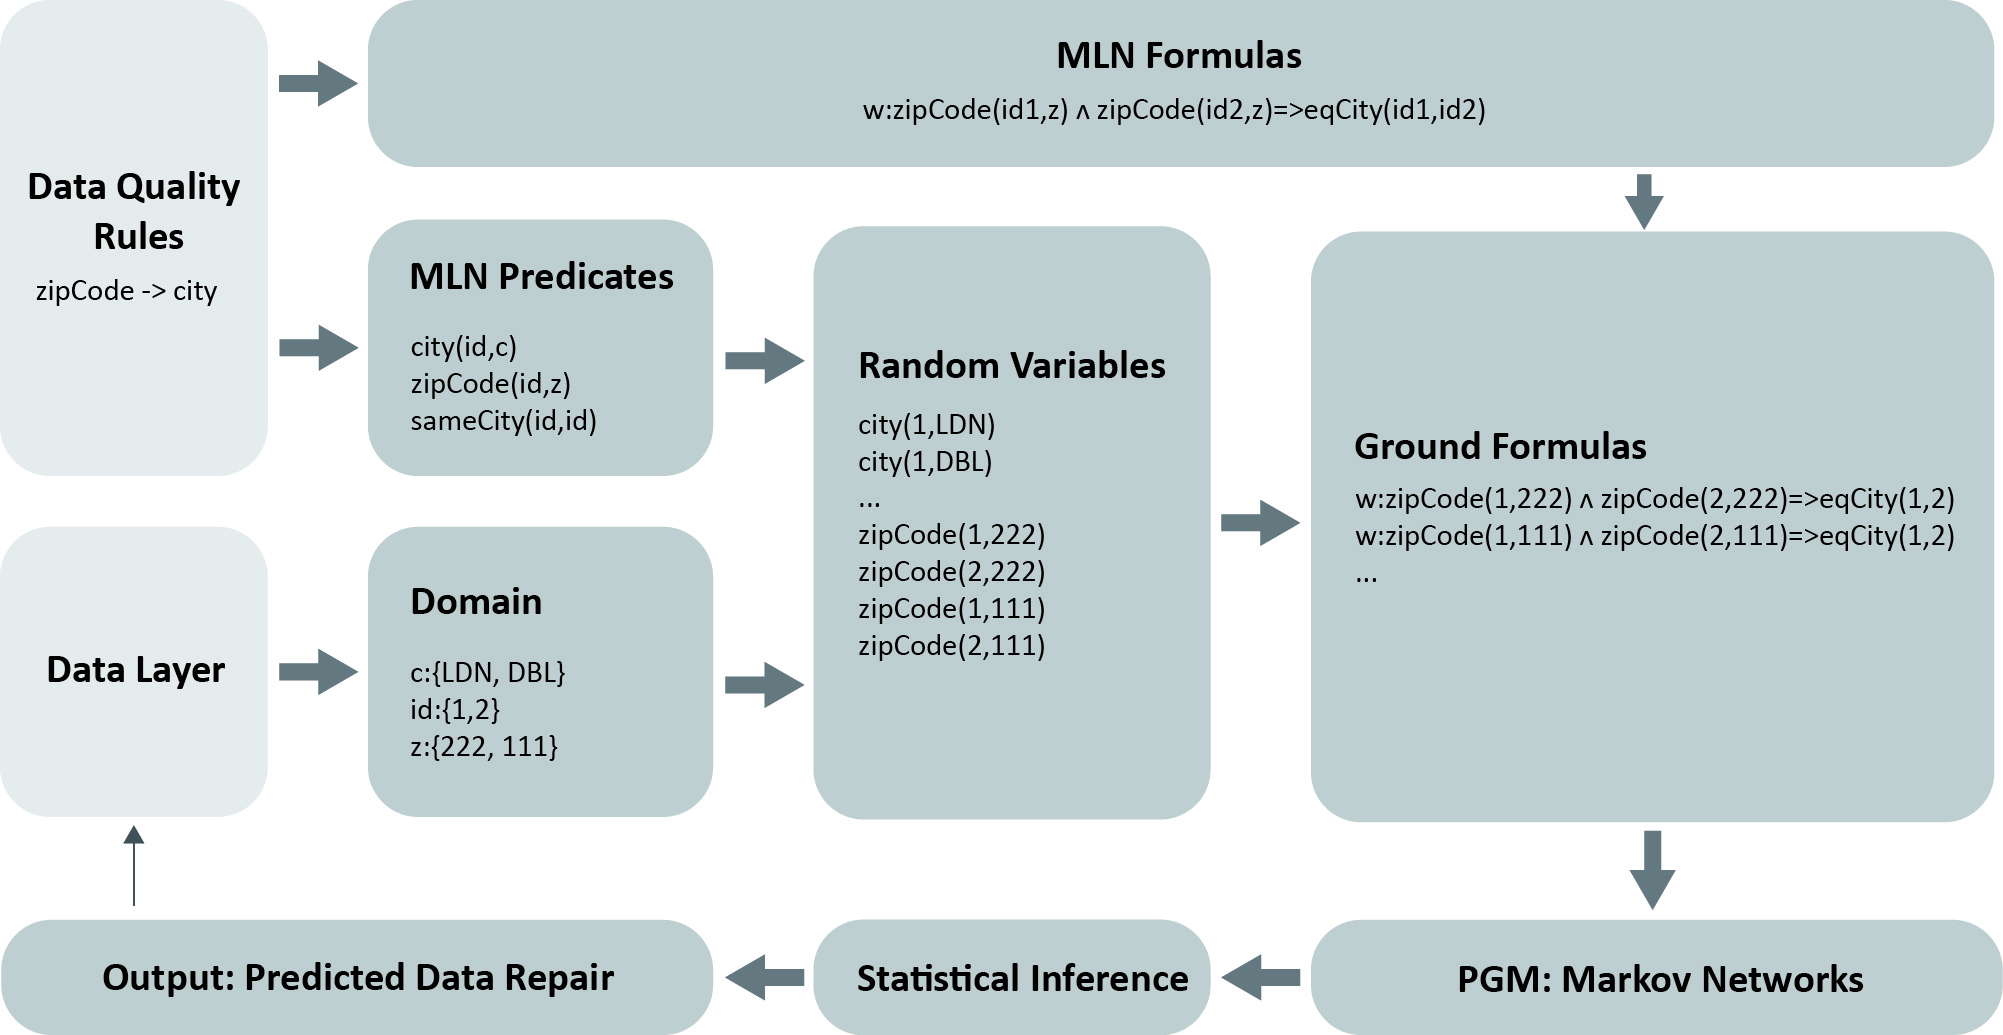
\includegraphics[width=450px, height=200px]{img/mlogic-grounging.jpg}
 \caption{\anno{Please redo this picture to make it look better} Markov Logic Network grounding process constists of two phases 1) MLN definintion by fixing MLN schema, domain and weighted formulas; 2) MLN instantiation by assigning truth values to the all possible instantiations of the MLN predicates and using these ground atoms in formulas.}
 \label{fig:mlngrounding}
\end{figure*}

\subsection{Compilation of Data Cleaning Rules to Predicate Calculus}
\label{sec:ml}

\anno{Does your system automate the compilation? If yes, mention this!} Next, we describe how to connect the Data Quality Rules formalism to the Markov logic. The base of Markov logic programs is predicate calculus \cite{genesereth1987logical}, because Markov logic consists of first-order logic sentences. Therefore, we describe a general method to compile formal constraint based data cleaning rules into predicate calculus. We define data cleaning rules in the form of CFDs and MDs as introduced in Section~\ref{sec:expl}. For example, given the following functional dependency $\phi: X \rightarrow Y$, according to the~\cite{Fagin:1982:HCD:322344.322347}, we express $\phi$ as \textit{first-order logic} sentence:
\begin{equation}
\mathsf{\forall x, y_1, y_2, z_1, z_2 \mathcal{R}(x, y_1, z_1) \wedge \mathcal{R}(x, y_2, z_2) \Rightarrow y_1=y_2}
\label{fd2fol}
\end{equation}

This first-order logic sentence is crucial for compilation of data cleaning rules into predictive models. \note{Aha, why?} Consider the logical equivalence of the data quality rule $\phi$ in \ref{fd2fol} as a composite component, consisting of subcomponents such as atomic sentences (attribute), logical and quantified sentences (RHS and LHS in FD $\phi$). To describe the structure of $\phi$ in a predicate calculus, we choose symbols that designate the elements of our conceptualization. In connection to the fundamentals of data quality management (c.f.,~Section~\ref{sec:expl}), we define the \textit{vocabulary} we use for the compilation of data quality rules: 
%\anno{WHY ANOTHER VOCABULARY? THIS IS SUPER CONFUSING!!! REWRITE THIS PART TO CONNECT TO THE REST OF THE PAPER}

The \textit{Universe of Disclosure} is specified by the set of all objects from domain $dom(U)$ that is fixed for the set of attributes $attr(\mathcal{R})$. A \textit{term} is used as a name for an object in the universe of discourse. We define \textit{variables} to denote arguments in atoms and \textit{constants} to denote data constants of particular domain $dom(U_i)$ of an $i$-th attribute $U_i \in attr(\mathcal{R})$. To designate the tuple in relation $\mathcal{R}$: $\mathcal{R}(x_1,x_2, \dots , x_n)$, we use atomic sentences $\mathsf{\textsf{attr-X}_1(id,v_1)}$, $\mathsf{\textsf{attr-X}_2(id,v_2)}$ $\dots$ $\mathsf{\textsf{attr-X}_n(id,v_n)}$ where $\mathsf{\textsf{attr-X}_i(id,v_i)}$ means that $\mathsf{v_i}$ is a attribute value of the $i$-th attribute in $\mathcal{R}(x_1,x_2, \dots , x_n)$ of the $id$-th tuple in relation $\mathcal{R}$. \textit{Relation Constants} denote relations between several objects:
	\begin{itemize}
		\item Similarity: $\mathsf{\textsf{similar}(x_1,x_2)}$ means that $\mathsf{x_1}$ similar to $\mathsf{x_2}$ (e.g by using different similarity measures like cosine or jaccard similarities).
		\item Equality: $\mathsf{\textsf{equal-X}(id_1, id_2)}$ means that the values of the attribute X of two tuples $\mathsf{id_1}$ and $\mathsf{id_2}$ should be equal.
		\item Matching: $\mathsf{\textsf{match-X}(id_1, id_2)}$ means that values of two tuples $\mathsf{id_1}$ and $\mathsf{id_2}$ of the attribute X are identified to match.
		\item Custom Predicate: used for encoding diverse semantic constraints (e.g. \textit{contains}, \textit{between}, \textit{less} etc.), which are not part of the data constraints.
	\end{itemize}

%\note{Is the compilation more than a slightly different syntax? What are the challenges? This is one of the contributions, need more elaboration.} this is formalization, previous reviewer has asked for.
Given this vocabulary, we describe our conceptualization of the data quality rules with predicate-calculus sentences. For example, for the functional dependency $\phi: X \rightarrow Y$ and the first-order logic sentence in Formula \ref{fd2fol}, we compile to the corresponding Markov logic formula as follows:
\begin{flalign*}
  & \mathsf{\textsf{attr-X}(id_1, x) \wedge \textsf{attr-X}(id_2, x) \Rightarrow \textsf{equal-Y}(id_1, id_2)} & 
\end{flalign*}
\vspace*{-0.5cm}

Analogously, we translate a matching dependency $ \mu: \mathcal{S}_1[x_1]\approx \mathcal{S}_2[x_2]\rightarrow \mathcal{S}_1[y_1]\rightleftharpoons \mathcal{S}_2[y_2]$ on a database instance $\mathcal{D}$ with two relational schemas $\mathcal{S}_1$ and $\mathcal{S}_2$ as follows:
\begin{flalign*}
  & \mathsf{\textsf{attr-X/S1}(id_1, x_1) \wedge \textsf{attr-X/S2}(id_2, x_2) \wedge \textsf{similar}(x_1, x_2)} & \\
  & \mathsf{\Rightarrow \textsf{S1/match-Y/S2}(id_1, id_2)} & 
\end{flalign*}
\vspace*{-0.5cm}

If we specify a matching dependency using two relations, we need to mark the attributes corresponding to a relation with that relation $\mathsf{\textsf{attr-X/}}\mathcal{R}$. Furthermore, as introduced above, we use predicates to represent operators in the data quality as shown in Table \note{ref table}.

\begin{table}[h]\footnotesize
%\scriptsize
\centering
\begin{tabular}{@{}lcl@{}}
\toprule
Concept    & Operator & Predicate \\ \midrule
Similarity & $\mathcal{S}_1[x_1]\approx \mathcal{S}_2[x_2]$        & $\mathsf{\textsf{similar}(x_1,x_2)}$ \\
Equality   & $y_1=y_2$ & $\mathsf{\textsf{equal-Y}(id_1, id_2)}$ \\
Matching   & $\mathcal{S}_1[y_1]\rightleftharpoons \mathcal{S}_2[y_2]$   & $\mathsf{\textsf{S1/match-Y/S2}(id_1, id_2)}$ \\ \bottomrule
\end{tabular}
\note{give table a name}
\end{table}

%\anno{TOO GENERIC AND HIGH LEVEL, SOUNDS LIKE A COPY FROM AN ML TEXTBOOK. CONNECT THIS TO OUR PROBLEM! -> this is not a copy from any books.
% but you are correct, this should be connected to the backend of the method.
%MLNs are created by writing a set of first-order logic rules with weights, constructed using variables that range of objects in the domain of interest and predicates that represent relations between these objects. Predicates can be observed or hidden. \textit{Observed predicates} are relations between objects that can be seen in a given data set. $\mathsf{\textsf{attr-X}_1(id,v_1)}$, $\mathsf{\textsf{attr-X}_2(id,v_2)}$ $\dots$ $\mathsf{\textsf{attr-X}_n(id,v_n)}$  where $\mathsf{\textsf{attr-X}_i(id,v_i)}$ are observed predicates. In addition, an MLN may have a number of \textit{hidden predicates}, meaning that they are not observed in the input data, but can be inferred through rules. In our case, $\mathsf{\textsf{equal-Y}(id_1, id_2)}$ and $\mathsf{\textsf{S1/match-Y/S2}(id_1, id_2)}$ are hidden.  The goal of probabilistic inference is to infer the likelihood for observed and hidden predicates given a rule set and evidence. We define the MLN in such a way that reasoning about hidden predicates given evidence and data cleaning rules allows us to determine data repair operations.}

%\subsubsection{First-Order Logic Formulae}
%\note{Explain why we are doing all of this? What is the advantage?} 
We assume that integrity constraints have been already determined by using methods reviewed in \cite{liu2012discover} or specified by domain experts manually. To demonstrate the compilation of the data cleaning rules into Markov Logic, have a look at the CFD from the motivation example in Section~\ref{sec:expl}. This CFD states that if any two tuples agree on attribute values for $\mathsf{\textsf{city}}$ and $\mathsf{\textsf{phone}}$, then the attribute values on $\mathsf{\textsf{street}}$ and $\mathsf{\textsf{zip}}$ should agree as well:
\begin{equation*}
\mathsf{fd: \textsc{transaction}([\textsf{city}, \textsf{phone}] \rightarrow [\textsf{street}, \textsf{zipcode}])}
\end{equation*}
\vspace*{-0.5cm}

To enable straightforward compilation, we assume that CFDs are provided in the normal form. This means if $\psi(X \rightarrow Y_1,Y_2,\dots , T_p)$, then $\psi$ will be decomposed into several CFDs where $RHS(\psi)$ (right hand side of $\psi$) becomes a single attribute: $\psi_1(X \rightarrow Y_1 , T_p)$, $\psi_2(X \rightarrow Y_2 , T_p) \dots$. Following the normalization rule for functional dependencies, we split the $\mathsf{fd}$ rule into two:
\begin{flalign*}
& \mathsf{cfd_1: \textsc{transaction}([\textsf{city}, \textsf{phone}] \rightarrow [\textsf{street}], t_1=(\_, \_ \parallel  \_))}& \\
& \mathsf{cfd_2: \textsc{transaction}([\textsf{city}, \textsf{phone}] \rightarrow [\textsf{zipcode}], t_2=(\_, \_ \parallel  \_))}&
\end{flalign*}
\vspace*{-0.5cm}

According to~\cite{Fagin:1982:HCD:322344.322347} we can represent these $\mathsf{cfd_1}$ and $\mathsf{cfd_2}$ as two first-order logic formulae:
\begin{flalign*}
& \mathsf{1)~\forall~\textsf{city}, \textsf{phone}, \textsf{street}_1, \textsf{street}_2 }& \\
& \mathsf{\textsc{transaction}(\textsf{city}, \textsf{phone}, \textsf{street}_1)~\wedge~\textsc{transaction}(\textsf{city}, \textsf{phone}, \textsf{street}_2) }& \\
& \mathsf{ \Rightarrow \textsf{street}_1=\textsf{street}_2 }& \\
& \mathsf{2) ~\forall~\textsf{city}, \textsf{phone}, \textsf{zip}_1, \textsf{zip}_2 }& \\
& \mathsf{ ~\textsc{transaction}(\textsf{city}, \textsf{phone}, \textsf{zip}_1) \wedge~\textsc{transaction}(\textsf{city}, \textsf{phone}, \textsf{zip}_2) }& \\
& \mathsf{ \Rightarrow \textsf{zip}_1=\textsf{zip}_2 }&
\end{flalign*}
\vspace*{-0.5cm}

In words, the formulas state that if two tuples of the \textsc{transaction} relation agree on the \textsf{city} and \textsf{phone} values, then their \textsf{street} and \textsf{zip} values should be the same. Once we have formulated our integrity constraints as first-order logic formulas, we translate them into Markov
Logic syntax. We illustrate this with the first-order logic formulae $\mathsf{1)}$ and $\mathsf{2)}$ defined above.
Given that every attribute from the schema $\mathsf{\textsc{transaction}}$ is expressed as a predicate, we need two predicates, 
namely $\mathsf{\textsf{city}(id, city)}$ and $\mathsf{\textsf{phone}(id, phone)}$ to encode the LHS of $\mathsf{fd}$ . They indicate the values for the fields \textsf{city} and \textsf{phone} for each tuple. The full example is given in Table~\ref{tab:mlndeclare}, which shows all steps in predicate translation and how data from our example database is translated into grounded atoms. Additionally, we define two predicates for our data quality rule, namely $\mathsf{\textsf{equal-street}(id, id)}$ and $\mathsf{\textsf{equal-zip}(id, id)}$. These predicates model equality of two values of the attribute \textsf{street} respectively \textsf{zip} (as denoted by the $\mathsf{fd}$ rule above):
\begin{flalign*}
	& \mathsf{1)  \textsf{city}(id_1, city) \wedge \textsf{city}(id_2, city) \wedge \textsf{phone}(id_1, phone) }& \\ 
	& \mathsf{  \wedge \textsf{phone}(id_2, phone) \Rightarrow \textsf{equal-street}(id_1, id_2)} & \\
	& \mathsf{2)  \textsf{city}(id_1, city) \wedge \textsf{city}(id_2, city) \wedge \textsf{phone}(id_1, phone) }& \\ 
	& \mathsf{  \wedge \textsf{phone}(id_2, phone) \Rightarrow \textsf{equal-zip}(id_1, id_2)} & 
\end{flalign*}
\vspace*{-0.5cm}

Please note that using the same arguments in predicates $\mathsf{\textsf{city}(id, city)}$ and $\mathsf{\textsf{phone}(id, phone)}$ encodes equality of the corresponding values in Markov logic program. The two different tuples are distinguished by $\mathsf{id_1}$ and $\mathsf{id_2}$. 
The data quality rules form the basis for a Markov Logic program. A particular advantage of Markov Logic is its \textit{modularity} while modeling. We can create "complex" statistical models by combining various "atomic" models. Thereby, we consider each declared data quality rule as an "atomic" probabilistic model. In combination, these small models form a "compound" model. So far we have shown how to express integrity constraints in terms of predicate calculus.
Having declared the data quality rules by capturing all correlations and constraints, we can now infer potential predicates, such as $\mathsf{\textsf{equal-street}(id, id)}$. This predicate holds the information about possible repairs on the attribute $\mathsf{\textsf{street}}$ in the \textsc{transactions} tables in our running example from Section~\ref{sec:expl}. Reasoning about such hidden predicates allows us to decide which attributes get a particular repair. 

\begin{table}[t]\footnotesize
%\scriptsize
\centering
\begin{tabular}{@{}ll@{}}
\toprule
Phase                                                                             & Example                                                                                                                                                          \\ \midrule
1) Schema definition                                                              & \begin{tabular}[c]{@{}l@{}}$t_2$(item, firstname, lastname, street,\\ city, zipcode, phone)\end{tabular}                                                              \\ \midrule
\begin{tabular}[c]{@{}l@{}}2) Observed predicates \\ MLN declaration\end{tabular} & \begin{tabular}[c]{@{}l@{}}$\mathsf{\textsf{firstname}(id, value)}$ \\ $\mathsf{\textsf{lastname}(id, lastname)}$ \\ $\mathsf{\textsf{street}(id, street)}$ \\ $\mathsf{\textsf{city}(id, city)}$\\ $\mathsf{\textsf{zip}(id, code)}$ \\ $\mathsf{\textsf{phone}(id, num)}$\end{tabular} \\ \midrule
3) Data                                                                           & \begin{tabular}[c]{@{}l@{}}$t_2$(Galaxy 5, NULL, Miller, \\ 12 Hay St., NULL, 818, 11234)\end{tabular}                                                              \\ \midrule
4) Grounded (evidence) atoms                                                      & \begin{tabular}[c]{@{}l@{}} $\mathsf{\textsf{item}(2, Galaxy5)}$ \\ $\mathsf{\textsf{lastname}(2, Miller)}$ \\ $\mathsf{\textsf{street}(2, 12HaySt.)}$ \\ $\mathsf{\textsf{zip}(2, 818)}$ \\ $\mathsf{\textsf{phone}(2, 11234)}$\end{tabular}                         \\ \bottomrule
\end{tabular}
\caption{\label{tab:mlndeclare} MLN declaration process and creation of grounded atoms for tuple 2 in the \textsc{Transactions} example table.}
\end{table}
\subsection{Data Repair as Joint Inference}
\label{subsec:jointinference}
%\anno{REWRITE THIS FIRST PARAGRAPH TO MAKE IT CLEAR:}
Markov logic defines a knowledge representation system that combines first-order logic as a declarative language with probabilistic graphical models (undirected Markov Networks MLNs) on top of which we perform probabilistic inference. Semantically, a MLN is a log-linear model, which defines the probability distribution over possible worlds, in our case all possible states in the database.

We create MLNs by writing a set of first-order logic rules (c.f.,~Section~\ref{sec:ml}) with weights by using predicates that represent relations between these objects. We distinguish between observed and hidden predicates. \textit{Observed predicates} are relations between objects which exist in a given dataset: $\mathsf{\textsf{attr-X}_1(id,v_1)}$, $\mathsf{\textsf{attr-X}_2(id,v_2)}$ $\dots$ $\mathsf{\textsf{attr-X}_n(id,v_n)}$ are observed predicates, which encode that $\mathsf{\textsf{attr-X}_i}$ has value $\mathsf{v_i}$ on tuple $\mathsf{id}$. In addition, an MLN may have a number of \textit{hidden predicates}, which are not present in the input data, but can be inferred through rules. In our case, $\mathsf{\textsf{equal-Y}(id_1, id_2)}$ and $\mathsf{\textsf{S1/match-Y/S2}(id_1, id_2)}$ are hidden.  The goal of probabilistic inference is to infer the likelihood for observed and hidden predicates given a rule set and evidence. We define the MLN in such a way that reasoning about hidden predicates given evidence and data cleaning rules allows us to determine data repair operations. In other words, we perform inference task as a prediction for the data cleaning.

%%%%%%
An important step in our method is \textit{grounding} of the MLN (in details illustrated in Figure \ref{fig:mlngrounding} \note{EXPLAIN THIS FIGURE IN DETAIL *PEITSCH*}). Because constraint-based rules are data agnostic~\cite{fan2012foundations}, we need to ``ground'' previously defined predicates with the available evidence, in our case the database to process. We take the content of the database (a set of tuples) and produce a set of observed predicates (so-called \textit{grounded atoms}). Let $n$ denote the number of schema attributes. Then we convert each tuple from the database into $n$ different Markov Logic evidence atoms. For example, we translate transaction 2 in our running example into the following 6 grounded atoms: \textsf{item}(2, Galaxy 5), \textsf{firstname}(2, Max), \textsf{lastname}(2, Miller), \textsf{street}(2, 12 Hay St.), \textsf{zip}(2, 818) and \textsf{phone}(11234). These are examples of observed predicates for the dataset. Table~\ref{tab:mlndeclare} summarizes the process of the groundings creation. We use these groundings (or evidence atoms) in the joint inference for data cleaning. 
%%%%%


%\anno{CONFUSING, REWRITE OR REMOVE: Markov Networks can be viewed in terms of \emph{cliques} which are subgraphs where all pairs of nodes are connected.} Edges between nodes are parametrized by so-called potentials, to encode the strength of a conditional dependency. \note{What do edges and nodes represent?} \anno{CONFUSING, REWRITE OR REMOVE: The joint probability of a Markov Network is attained by computing the normalized product over clique potentials.} 
%\todo[inline]{markov logic into from the Rockit paper section: "Markov Logic"; \\ also explain $F_i$ below - adopt from ELEMENTARY paper page 7: semantics}
%Semantically, a Markov Logic Network (MLN) is a log-linear model, which defines the probability  distribution over possible worlds, in our case all possible states in the database.% Such models have many names, including maximum-entropy models, exponential models, and Gibbs models; Markov random fields are structured log-linear models, conditional random fields (Lafferty et al., 2001) are Markov random fields with a specific training criterion

%We consider a set of formulae $\bar{F} = F_1, F_2 \dots F_N$ with corresponding weights $w_1 \dots w_N$ as an input. \note{Why? What do these formulas represent?} These weighted first-order logic formulae define a probability distribution as follows: $P \left( X = x \right) = \frac{1}{Z} \exp\left( \sum_{F_i} w_i n_i \left( x \right) \right)$. Here, $n_i(x)$ denotes the number of true groundings of formula $F_i$ in $x$. The term $w_i$ represents the corresponding formula weight and $Z$ is a normalization constant. Given a formula $F_i$ with variables $(x_1 \dots x_n)$, we create new formula $g$ called \textit{ground formula} \note{Why?} as follows: for each $x_k$ and its domain $dom(U_k)$, each variable $x_k$ is being substituted with a value from its domain $dom(U_k)$. Let $w$ be a function that maps each ground formula $g$ to its assigned weight. If $g$ is false (true) and $w(g)>0$ (respectively $w(g)<0$), then the ground formula is violated. Hence, the probability of the particular world is higher the less ground formulae is violated and the lower is the cost of the world $W$: \note{Don't talk about 'worlds', connect this to our task}. $cost_W = \sum_{g \in V(W)} w(g)$. Here $V(W)$ denotes the set of violated ground formulae.

%\anno{CONFUSING, REMOVE: Please note that formula weights are not probabilities itself but the certainty of this formula. This also means that weights can be considered as empirical frequencies where each formula should hold. Weights can be specified in two ways: first, heuristically (e.g using the domain expertise); second, by performing weight learning on data, e.g. by running weight learning algorithms on MLN \cite{lowd2007efficient}.}

%\note{CLARIFY: In this paper we focus on an inference task as a prediction for the data cleaning operations.} moved to another place.


%\todo[inline]{Manu: there is an example there.. so explain that with some probabilistic formulae and the corresponding PGM drawn out}
%\anno{REMOVE AND REPLACE WITH A SINGLE SENTENCE: The main advantage of Markov logic is the ability to reason about complex and interacting relationships, such as different data quality issues. The query computation is also known as \textit{inference}. In addition, through the cleaning rules that we have defined in the Rule-based Data Quality Management component of our system, there are a number of hidden predicates we use for data repair. The Statistical Processing component of our system (see Figure~\ref{fig:mlngrounding} for an overview) executes probabilistic inference to determine probable groundings for the hidden predicates. This component takes as input both the Markov Logic Networks defined through component I, as well as the grounded atoms produced by component III from the available data. It then constructs a probabilistic graphical model using these inputs on top of which it performs probabilistic inference. Figure \ref{fig:mlngrounding} visualizes the MLN grounding process.}

%\anno{Where are we introducing more and more terminology? What are literals?} 
Given an MLN that models data cleaning rules, let $q \in \mathcal{L}^n$ denote a hidden predicate with $n$ \emph{literals} (random variables) $L_1,...,L_n$, where each literal $L_i$
has $2$ discrete states, $L_i = \lbrace 0,1 \rbrace$.
Then, the MLN is a joint distribution on  $L_1,...,L_n$ that 
is specified by a vector $\phi(q)$ of $d$ integer values, where
each element represents the number of true groundings of the 
corresponding literal in the formula and $d$ denotes the 
maximum number of literals in a given formula. Additionally, 
we have a weight/parameter vector $\theta \in \mathcal{R}^d$:
%\vspace{-3em}
\begin{equation*}
Pr \left( q | \theta \right) = 
\frac{1}{Z(\theta)} \exp\left( \langle \theta, \phi(q) \rangle  \right), 
Z(\theta) = \sum_{q \in \mathcal{L}^n}\exp\left( \langle \theta, \phi(q) \rangle  \right) 
\end{equation*}
%\vspace{-2em}
where $\langle \theta, \phi(q) \rangle$ denotes a dot product. 
$Z(\theta)$ is the normalization constant also called the 
\emph{partition function}. Since the partition function is a constant and the exponential is monotonic, finding the MAP assignment in our data cleaning problem is equivalent to finding the assignment $q_M$ that maximizes the probability $Pr \left( q | \theta \right)$.

The output of the inference are data repair operations; for example, the hidden predicate \textsf{equal-street} may be determined to have (among other groundings) the following likely value: $\mathsf{\textsf{equal-street}(1, 3)}$, indicating that the \textsf{street} field for transaction 3 should have the same value as the \textsf{street} field of transaction 1. In this case, the data repair operation is to replace the \textsc{null} value in transaction 3 with the address ``1 Sun Dr.''. \note{Shouldn't the MLN allow us to inspect the uncertainty in these decisions? Can you elaborate on that?} As we noted in the discussion of the running example, there is an interplay of different rules that affect the probability of the hidden predicates. Therefore, the inference produces the most likely state of the entire Markov Logic Network with regards to all integrity constraints. The probabilities for the hidden predicates are therefore influenced by \textit{all} defined data quality rules. By running the inference over the entire database we predict the most likely data repairs for our data set by determining the most likely grounding of the hidden predicates and this reduces to computing \textsc{map} inference on the MLN model.      

The difficulty in designing algorithms for MAP inference arises when finding an efficient way to reason about the large number of possible assignments to the variables in the model. In terms of theoretical guarantees, inference is NP-hard and in many cases cannot even be approximated \note{reference please}. Amongst the numerous techniques that are available to solving MAP inference problems, we chose to cast the inference problem as an \emph{integer linear program} (ILP). Another competitive approach called \emph{message passing} perform \emph{belief propagation} along the edges of the graphical model. Although, message passing is easy to implement it has troubles converging \cite{schwing2011distributed, felzenszwalb2006efficient, pritch2009shift} and tends not to give as good results as ILP~\cite{NoessnerNS13}. 

